\documentclass[tikz,border=4pt]{standalone}
\usepackage{tikz}
\usetikzlibrary{arrows.meta}
\begin{document}
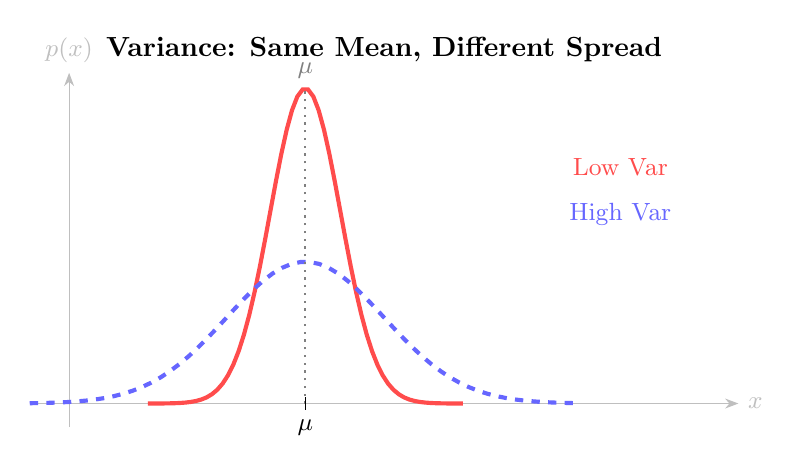
\begin{tikzpicture}[>=Stealth]
    \node[font=\bfseries] at (4,4.5) {Variance: Same Mean, Different Spread};

    % Axes
    \draw[->,gray!50] (-0.5,0) -- (8.5,0) node[right,font=\small] {$x$};
    \draw[->,gray!50] (0,-0.3) -- (0,4.2) node[above,font=\small] {$p(x)$};

    % Low variance (narrow, tall)
    \draw[red!70,line width=1.5pt,domain=1:5,samples=60]
        plot ({\x},{4*exp(-(\x-3)*(\x-3)/0.4)});

    % High variance (wide, short)
    \draw[blue!60,line width=1.5pt,dashed,domain=-0.5:6.5,samples=60]
        plot ({\x},{1.8*exp(-(\x-3)*(\x-3)/2)});

    % Mean line
    \draw[gray,dotted,line width=0.8pt] (3,0) -- (3,4)
        node[above,font=\small,gray] {$\mu$};

    % Tick
    \draw (3,0.08) -- (3,-0.08) node[below,font=\small] {$\mu$};

    % Legend
    \node[red!70,font=\small] at (7,3) {Low Var};
    \node[blue!60,font=\small] at (7,2.4) {High Var};
\end{tikzpicture}
\end{document}
